\subsection{Dynamic Airspace Sectorisation}

\Gls{DAS} is a responsive approach to airspace management that adjusts sector boundaries according to real-time traffic demand and capacity constraints \cite{Zhou_2023}.
By clustering traffic patterns to identify high-density areas, \gls{DAS} aims to support efficient planning and enhance controller operations \cite{Schultz_2018}.
% The key objective is to adapt sector configurations dynamically, in a time-dependent manner, to better match actual operational needs.

% Early research on optimising airspace structure applied \glspl{EA}, focusing on balancing controller workload through several operationally relevant metrics, such as the total and standard deviation of task load, geometric coherence of sector shapes and number of flight path intersections caused by sector boundaries \cite{Schultz_2018}.
% This approach successfully reproduced existing operational sector designs, such as those in the EDDYDUTA area (Figures \ref{airspace-normal} and \ref{airspace-das}), without relying on expert knowledge.
% It also demonstrated adaptability to fluctuating daily traffic patterns (Figure \ref{airspace-dynamic}).

Early research applied \glspl{EA} to optimise sector structures by balancing controller workload using metrics like task load distribution, geometric coherence, and flight path intersections. 
This method successfully replicated operational sector designs, such as those in the EDDYDUTA area (Figure~\ref{airspace}), and adapted to daily traffic variations without expert input \cite{Schultz_2018}.

\begin{figure}[!ht]
    \centering
    \begin{subfigure}{.45\textwidth}
        \centering
        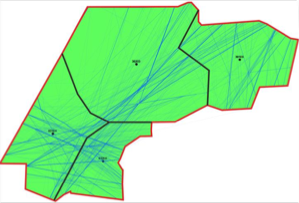
\includegraphics[width=.7\textwidth]{img/airspace.png}
        \caption{Original airspace structure}
        \label{airspace-normal}
    \end{subfigure}
    \begin{subfigure}{.45\textwidth}
        \centering
        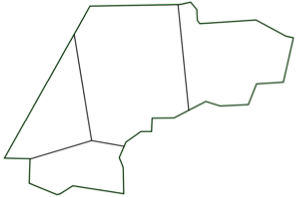
\includegraphics[width=.7\textwidth]{img/airspace-das.png}
        \caption{Sectorisation after \gls{DAS} optimisation}
        \label{airspace-das}
    \end{subfigure}

    \begin{subfigure}{\textwidth}
        \centering
        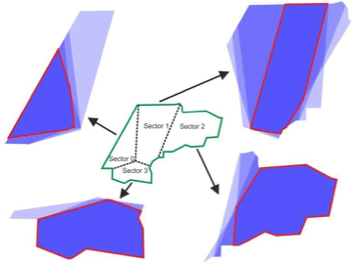
\includegraphics[width=.5\textwidth]{img/airspace-dynamic.png}
        \caption{Dynamic adaptation to traffic demand}
        \label{airspace-dynamic}
    \end{subfigure}

    \caption{Airspace EDDYDUTA \cite{Schultz_2018}}
    \label{airspace}
\end{figure}

Recent advancements explore deep learning to improve \gls{DAS}. 
Zhou et al. \cite{Zhou_2022} introduced a \gls{MTL} model with \gls{Bi-LSTM} networks to predict traffic flow and capacity, enabling proactive sector adjustments based on traffic-capacity imbalance forecasts across multiple time horizons. 
However, the model's black-box nature limits operational trust.

% Recent research explores deep learning to enhance \gls{DAS}, offering greater scalability and predictive accuracy than traditional \glspl{EA}.
% Zhou et al. \cite{Zhou_2022} introduced a \gls{MTL} model using \gls{Bi-LSTM} networks to predict both traffic flow and airspace capacity. 
% This model supports proactive sector adjustments based on traffic-capacity imbalance forecasts across multiple time horizons.
% While effective, the \gls{Bi-LSTM} model is a black-box system, which limits its operational acceptability due to the lack of transparency in how predictions are derived.

To improve interpretability, Zhou et al. \cite{Zhou_2023} proposed AirFusion, a transparent \gls{AI} framework using the \gls{TFT} for time-series forecasting. 
It predicts demand and capacity up to four hours ahead, respects controller constraints, and uses \gls{DBSCAN} clustering and weighted graphs to guide sectorisation. 
AirFusion achieves high predictive accuracy (mean errors: 0.0234 for demand, 0.0291 for capacity) with strong R-squared values (0.9133 and 0.9605).
Figure~\ref{airspace-tft} illustrates the clustering and sector adaptation, where flight trajectories are colour-coded and major flows highlighted. 
When demand exceeds capacity, sectors are subdivided (purple dashed lines) to maintain workload balance.

% To address this, Zhou et al. \cite{Zhou_2023} proposed a more interpretable \gls{AI} framework called AirFusion, which integrates the \gls{TFT} for time-series forecasting.
% The model predicts airspace demand and capacity up to four hours in advance while respecting operational constraints imposed on air traffic controllers.
% It incorporates \gls{DBSCAN} clustering to identify major traffic flows and constructs weighted graphs to inform sectorisation decisions.
% Results show high predictive accuracy, with mean errors of 0.0234 (demand) and 0.0291 (capacity), and R-squared values of 0.9133 and 0.9605, respectively.
% Clustering results are shown in Figure \ref{airspace-tft}, where flight trajectories are color-coded, and major flows within each cluster are indicated by thickened lines. 
% When demand exceeds sector capacity, sectors are subdivided (purple dashed lines) to maintain manageable workloads.

\begin{figure}[!ht]
    \centering
    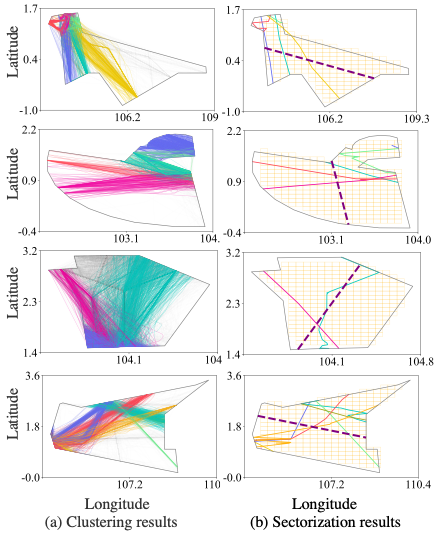
\includegraphics[width=.5\textwidth]{img/airspace-tft.png}
    \caption{Clustering and sectorisation results for selected sectors \cite{Zhou_2023}.}
    \label{airspace-tft}
\end{figure}

% Compared to the earlier \gls{Bi-LSTM} approach, the \gls{TFT}-based model offers better interpretability, thanks to integrated feature selection and attention mechanisms. 
% This makes it more suitable for operational deployment, where trust and explainability are critical for controller acceptance.

Compared to the earlier \gls{Bi-LSTM} model, AirFusion's integrated attention and feature selection mechanisms improve explainability, making it more suitable for real-world deployment where transparency is essential.

